% \vspace{-0.5cm}
\section{Experiment}\label{sec:experiment}
% \vspace{-0.3cm}
In our experiments, we aim to answer the following research questions:
\textbf{RQ1:} Can \ourmethod achieve state-of-the-art reasoning performance with balances between efficiency and effectiveness?
\textbf{RQ2:} Can \ourmethod eliminate hallucinations and conduct faithful reasoning?
\textbf{RQ3:} Can \ourmethod generalize to unseen KGs on the fly? 

% \vspace{-0.5cm}
% \vspace{-0.1cm}
\subsection{Experiment Setups}
% \vspace{-0.1cm}

\begin{table*}[]
    \centering
    \caption{Performance comparison with different baselines on the two KGQA datasets.}
    \label{tab:kgqa}
    % \vspace{-0.2cm}
    \resizebox{.6\textwidth}{!}{%
        \begin{tabular}{@{}c|l|cc|cc@{}}
            \toprule
            \multirow{2}{*}{Types}           & \multicolumn{1}{c|}{\multirow{2}{*}{Methods}} & \multicolumn{2}{c}{WebQSP} & \multicolumn{2}{c}{CWQ}                                 \\ \cmidrule(l){3-6}
                                             & \multicolumn{1}{c|}{}                         & Hit                        & F1                      & Hit           & F1            \\ \midrule
            \multirow{10}{*}{LLM Reasoning}  & Qwen2-0.5B \citep{qwen2}                      & 26.2                       & 17.2                    & 12.5          & 11.0          \\
                                             & Qwen2-1.5B  \citep{qwen2}                     & 41.3                       & 28.0                    & 18.5          & 15.7          \\
                                             & Qwen2-7B \citep{qwen2}                        & 50.8                       & 35.5                    & 25.3          & 21.6          \\
                                             & Llama-2-7B \citep{touvron2023llama}           & 56.4                       & 36.5                    & 28.4          & 21.4          \\
                                             & Llama-3.1-8B \citep{llama3}                   & 55.5                       & 34.8                    & 28.1          & 22.4          \\
                                             & GPT-4o-mini  \citep{gpt4o}                    & 63.8                       & 40.5                    & 63.8          & 40.5          \\
                                             & ChatGPT \citep{chatgpt}                       & 59.3                       & 43.5                    & 34.7          & 30.2          \\
                                             & ChatGPT+Few-shot \citep{brown2020language}    & 68.5                       & 38.1                    & 38.5          & 28.0              \\
                                             & ChatGPT+CoT \citep{wei2022chain}              & 73.5                       & 38.5                    & 47.5          & 31.0              \\
                                             & ChatGPT+Self-Consistency  \citep{wangself}    & 83.5                       & 63.4                    & 56.0          & 48.1              \\ \midrule
            \multirow{5}{*}{Graph Reasoning} & GraftNet  \citep{sun2018open}                 & 66.7                       & 62.4                    & 36.8          & 32.7          \\
                                             & NSM \citep{he2021improving}                   & 68.7                       & 62.8                    & 47.6          & 42.4          \\
                                             & SR+NSM  \citep{zhang2022subgraph}             & 68.9                       & 64.1                    & 50.2          & 47.1          \\
                                             & ReaRev \citep{mavromatis2022rearev}           & 76.4                       & 70.9                    & 52.9          & 47.8          \\ 
                                             & \RE{UniKGQA \citep{jiang2022unikgqa}}                  & \RE{77.2}         & \RE{72.2}         & \RE{51.2}       & \RE{49.1}       \\\midrule
            \multirow{10}{*}{KG+LLM}         & KD-CoT \citep{wang2023knowledge}              & 68.6                       & 52.5                    & 55.7          & -             \\
                                             & EWEK-QA \citep{dehghan-etal-2024-ewek}        & 71.3                       & -                       & 52.5          & -             \\
                                             & ToG (ChatGPT)  \citep{sunthink}                 & 76.2                       & -                       & 57.6          & -          \\
                                             & ToG (GPT-4)  \citep{sunthink}                   & 82.6                       & -                       & 68.5          & -          \\
                                             & EffiQA \citep{dong2024effiqa}                 & 82.9                       & -                       & 69.5          &               \\
                                             & RoG (Llama-2-7B) \citep{luo2024rog}                        & 85.7                       & 70.8                    & 62.6          & 56.2          \\
                                             & GNN-RAG \citep{mavromatis2024gnn}             & 85.7                       & 71.3                    & 66.8          & 59.4          \\
                                             & GNN-RAG+RA \citep{mavromatis2024gnn}          & 90.7                       & 73.5                    & 68.7          & 60.4          \\ \cmidrule(l){2-6}
                                             & \ourmethod (Llama-3.1-8B + ChatGPT)                           & \textbf{92.6}              & 73.2                    & 72.7          & 60.9          \\
                                             & \ourmethod (Llama-3.1-8B + GPT-4o-mini)                       & 92.2                       & \textbf{74.1}           & \textbf{75.8} & \textbf{61.7} \\ \bottomrule
        \end{tabular}%
    }
    % \vspace{-0.7cm}
\end{table*}

\noindent\textbf{Datasets.} Following previous research \citep{luo2024rog,sunthink}, we first evaluate the reasoning ability of \ourmethod on two benchmark KGQA datasets: WebQuestionSP (WebQSP) \citep{yih2016value} and Complex WebQuestions (CWQ) \citep{talmor2018web}. Freebase \citep{bollacker2008freebase} is adopted as the knowledge graph for both datasets. To further evaluate the generalizability of \ourmethod, we conduct zero-shot transfer experiments on \RE{three new KGQA datasets: FreebaseQA \citep{jiang2019freebaseqa}, CSQA \citep{talmor2019commonsenseqa} and MedQA \citep{jin2021disease}. FreebaseQA adopts the same Freebase KG.} For CSQA, we use ConceptNet \citep{speer2017conceptnet} as the KG, while for MedQA, we use a medical KG constructed from the Unified Medical Language System \citep{yasunaga2021qa}.
%
The details of the datasets are described in \Cref{app:datasets}. 

\noindent\textbf{Baselines.} We compare \ourmethod with the 22 baselines grouped into three categories: 1) \emph{LLM reasoning methods}, 2) \emph{graph reasoning methods}, and 3) \emph{KG-enhanced LLM reasoning methods}. The detailed baselines are listed in \Cref{app:baselines}.

\noindent\textbf{Evaluation Metrics.} We adopt Hit and F1 as the evaluation metrics following previous works \citep{luo2024rog,sunthink} on WebQSP and CWQ. Hit checks whether any correct answer exists in the generated predictions, while F1 considers the coverage of all answers by balancing the precision and recall of predictions. Because CSQA and MedQA are multiple-choice QA datasets, we adopt accuracy as the evaluation metric.

\noindent\textbf{Implementations.} For \ourmethod, we use the KG-Trie to index all the reasoning paths within 2 hops starting from question entities. For the LLMs, we use a fine-tuned Llama-3-8B \citep{llama3} as the KG-specialized LLM. We generate top-10 reasoning paths and hypothesis answers from graph-constrained decoding. We adopt the advanced ChatGPT \citep{chatgpt} and GPT-4o-mini \citep{gpt4o} as the general LLMs for inductive reasoning. The detailed hyperparameters and experiment settings are described in \Cref{app:implementation}.

% Please add the following required packages to your document preamble:
% \usepackage{booktabs}
% \usepackage{multirow}
% \usepackage{graphicx}
\begin{table*}[]
    \centering
    \caption{Efficiency and performance comparison of different methods on WebQSP.}
    \label{tab:efficiency}
    % \vspace{-0.2cm}
    \resizebox{0.6\textwidth}{!}{%
    \begin{tabular}{@{}c|c|c|c|c|c@{}}
        \toprule
        Types                            & \multicolumn{1}{c|}{Methods} & Hit           & Avg. Runtime (s) & Avg. \# LLM Calls & Avg. \# LLM Tokens \\ \midrule
        \multirow{5}{*}{Retrieval-based} & S-Bert                       & 66.9          & 0.87             & 1                 & 293                \\
                                         & BGE                          & 72.7          & 1.05             & 1                 & 357                \\
                                         & OpenAI-Emb.                  & 79.0          & 1.77             & 1                 & 330                \\\cmidrule{2-6}
                                         & GNN-RAG                      & 85.7          & 1.52             & 1                 & 414                \\
                                         & RoG                          & 85.7          & 2.60             & 2                 & 521                \\ \midrule
        \multirow{2}{*}{Agent-based}     & ToG                          & 75.1          & 16.14             & 11.6              & 7,069              \\ 
        & EffiQA                    & 82.9         & -             & 7.3              & -              \\
        \midrule
        Ours                             & \ourmethod                   & \textbf{92.6} & 3.60             & 2                 & 231                \\ \bottomrule
        \end{tabular}%
    }
    % \vspace{-0.8cm}
\end{table*}

\subsection{RQ1: Reasoning Performance and Efficiency}\label{sec:kgqa}
\noindent\textbf{Main Results.}
In this section, we compare \ourmethod with other baselines on KGQA benchmarks to evaluate the reasoning performance. 
% We adopt the Llama-3.1-8B \citep{llama3} as the KG-specialized LLM and ChatGPT as well as GPT-4o-mini as the general LLM for \ourmethod. The results are shown in \Cref{tab:kgqa}.
%
From the results shown in \Cref{tab:kgqa}, \ourmethod achieves the best performance on both datasets, outperforming the second-best by 2.1\% and 9.1\%
in terms of Hit on WebQSP and CWQ, respectively. The results demonstrate that \ourmethod can effectively leverage KGs to enhance LLMs and achieve state-of-the-art reasoning performance.

Among the LLM reasoning methods, ChatGPT with self-consistency prompts demonstrates the best performance, which indicates the powerful reasoning ability inherent in LLMs. However, their performances are still limited by the model size and complex reasoning required over structured data. Graph reasoning methods, such as ReaRev, achieve competitive performance on WebQSP by explicitly modeling the graph structure. But they struggle to generalize across different datasets and underperform on CWQ. In KG+LLM methods, both agent-based methods (e.g., ToG, EffiQA) and retrieval-based methods (e.g., RoG, GNN-RAG) achieve the second-best performance. 
%
Nevertheless, they still suffer from inefficiency and reasoning hallucinations which limit their performance. In contrast, \ourmethod effectively eliminates hallucinations and conducts faithful reasoning by leveraging the structured KG index and graph-constrained decoding.

\noindent\textbf{Efficiency Analysis.}
To show the efficiency of \ourmethod, we compare the average runtime, number of LLM calls, and number of input tokens with retrieval-based and agent-based methods in Table \ref{tab:efficiency}. For retrieval-based methods, we compare with dense retrievers (e.g., S-Bert \citep{reimers-2019-sentence-bert}, BGE \citep{llm_embedder}, OpenAI-Emb. \citep{openai-embedding}) and graph-based retrievers (e.g., GNN-RAG \citep{mavromatis2024gnn}, RoG \citep{luo2024rog}), which retrieve reasoning paths from KGs and feed them into LLMs for reasoning answers. For agent-based methods, we compare with ToG \citep{sunthink} and EffiQA\footnote{Since there is no available code for EffiQA, we directly copy the results from the original paper.} \citep{dong2024effiqa}, which heuristically search on KGs for answers. The detailed settings are described in \Cref{app:implementation}.

Dense retrievers are most efficient in terms of runtime and LLM calls as they convert all paths into sentences and encode them as embeddings in advance. However, they sacrifice their accuracy in retrieving as they are not designed to encode graph structure. Graph-based retrievers and agent-based methods achieve better performance by considering graph structure; however, they require more time and LLM calls. Specifically, the retrieved graph is fed as inputs to LLMs, which leads to a large number of input tokens. Agent-based methods, like ToG, require more LLM calls and input tokens as the question difficulty increases due to their iterative reasoning process. 
In contrast, \ourmethod achieves the best performance with a reasonable runtime and number of LLM calls. With the help of KG-Trie, \ourmethod explores multiple reasoning paths at the same time during the graph-constrained decoding, which does not involve additional LLM calls or input tokens and benefits from the parallel GPU computation with low latency. More efficiency analysis under different beam sizes used for graph-constrained decoding can be found in parameter analysis.

% \begin{wraptable}{r}{0.6\textwidth}
\begin{table}
    \centering
    \vspace{-0.4cm}
    \caption{Ablation studies of \ourmethod on two KGQA datasets.}
    \label{tab:ablation}
    % \vspace{-0.3cm}
    \resizebox{1\columnwidth}{!}{%
    \begin{tabular}{@{}l|ccc|ccc@{}}
    \toprule
    \multicolumn{1}{c|}{\multirow{2}{*}{Variants}} & \multicolumn{3}{c|}{WebQSP}                   & \multicolumn{3}{c}{CWQ}                       \\ \cmidrule(l){2-7} 
    \multicolumn{1}{c|}{}                          & F1            & Precision     & Recall        & F1            & Precision     & Recall        \\ \midrule
    \ourmethod (Llama-3.1-8B + ChatGPT)                                    & \textbf{73.2} & \textbf{80.0} & \textbf{76.9} & \textbf{60.9} & \textbf{61.1} & \textbf{66.6} \\
    \ourmethod $w/o$ KG-specialized LLM            & 52.9          & 66.3          & 50.2          & 37.5          & 40.8          & 37.9          \\
    \ourmethod $w/o$ General LLM                   & 57.0          & 58.0          & 70.1          & 39.4          & 32.8          & 64.3          \\ \bottomrule
    \end{tabular}%
    }
    % \vspace{-.2cm}
\end{table}
    % \end{wraptable} 
\noindent\textbf{Ablation Study.} We first conduct an ablation study to analyze the effectiveness of the KG-specialized LLM and general LLM in \ourmethod. As shown in \Cref{tab:ablation}, the full \ourmethod achieves the best performance on both datasets. By removing the KG-specialized LLM, we feed all 2-hop reasoning paths into the general LLM. This results in a significant performance drop, indicating its importance in utilizing reasoning ability to find relevant paths on KGs for reasoning. On the other hand, removing the general LLM and relying solely on answers predicted by KG-specialized LLM leads to a noticeable decrease in precision, due to noises in its predictions. This highlighting the necessity of the general LLM for conducting inductive reasoning over multiple paths to derive final answers.


\noindent\textbf{Different LLMs.} We further analyze LLMs used for KG-specialized and general LLMs in \Cref{tab:different_llms}. For KG-specialized LLMs, we directly plug the KG-Trie into different LLMs to conduct graph-constrained decoding and use \RE{ChatGPT as the} general LLM for final reasoning. For general LLMs, we adopt the same reasoning paths generated by KG-specialized LLMs to different LLMs to produce final answers. For zero-shot and few-shot learning, we adopt the original LLMs without fine-tuning, whose prompt templates can be found in \Cref{fig:path_gen_prompt,fig:few_shotpath_gen_prompt}.
%\reza{Reza: When fine-tuning, what's the training data and the training objective?}

% Please add the following required packages to your document preamble:
% \usepackage{booktabs}
% \usepackage{multirow}
% \usepackage{graphicx}
% \begin{wraptable}{r}{0.65\columnwidth}
\begin{table}
    \centering
    % \vspace{-0.5cm}
    \caption{Comparison of different LLMs used in \ourmethod.}
    \label{tab:different_llms}
    % \vspace{-0.3cm}
    \resizebox{.9\columnwidth}{!}{%
        \begin{tabular}{@{}c|c|l|c|c@{}}
            \toprule
            Components                          & Learning Types                 & \multicolumn{1}{c|}{Variants} & Hit            & F1             \\ \midrule
            \multirow{9}{*}{\shortstack{KG-specialized\\LLM}} & \multirow{2}{*}{Zero-shot}  & Llama-3.1-8B                  & 28.25          & 10.32           \\
                                                &                             & Llama-3.1-70B                 & 38.53          & 12.53          \\ \cmidrule(l){2-5}
                                                & \multirow{2}{*}{Few-shot}   & Llama-3.1-8B                  & 33.24          & 11.19          \\
                                                &                             & Llama-3.1-70B                 & 41.13 & 13.14 \\ \cmidrule(l){2-5}
                                                & \multirow{5}{*}{Fine-tuned} & Qwen2-0.5B                    & 87.48 & 60.03          \\
                                                &                             & Qwen2-1.5B                    & 89.21          & 62.97          \\
                                                &                             & Qwen2-7B                      & 92.31          & 72.74          \\
                                                &                             & Llama-2-7B                    & 92.55          & \textbf{73.23} \\
                                                &                             & Llama-3.1-8B                  & \textbf{92.74} & 73.14 \\ \midrule
            \multirow{5}{*}{General LLM}        & \multirow{5}{*}{Zero-shot}  & Qwen-2-7B                     & 86.32          & 67.59          \\
                                                &                             & Llama-3.1-8B                  & 90.24          & 71.19          \\
                                                &                             & Llama-3.1-70B                 & 89.85          & 71.47          \\
                                                &                             & ChatGPT                       & \textbf{92.55}          & 73.23          \\
                                                &                             & GPT-4o-mini                   & 92.23 & \textbf{74.05} \\ \bottomrule
        \end{tabular}%
    }
    % \vspace{-.3cm}
\end{table}
% \end{wraptable}
Results in \Cref{tab:different_llms} show that a lightweight LLM (0.5B) can outperform a large one (70B) after fine-tuning, indicating the effectiveness of fine-tuning in enhancing the ability of LLMs and make them specialized for KG reasoning.
However, the larger LLMs (e.g., 7B and 8B) still perform better than smaller ones, highlighting the importance of model capacity in searching relevant reasoning paths on KGs. Similar trends are observed in general LLMs where larger models (e.g., GPT-4o-mini and ChatGPT) outperform smaller ones (e.g., Qwen-2-7B and Llama-3.1-8B), showcasing their stronger inductive reasoning abilities. This further emphasizes the need of paring powerful general LLMs with lightweight KG-specialized LLMs to achieve better reasoning driven by both of them.


% \begin{wrapfigure}{r}{0.55\columnwidth}
%   \vspace{-10pt}
\begin{figure}[]
    \begin{center}
        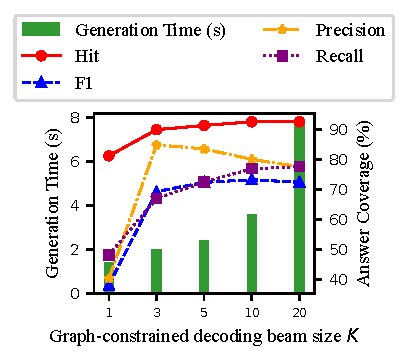
\includegraphics[width=.7\columnwidth]{images/k-beam.pdf}
      \end{center}
      \vspace{-20pt}
      \caption{Parameter analysis of beam size $K$.}
    \label{fig:beam-size}
    \vspace{-14pt}
\end{figure}
% \end{wrapfigure}
\noindent\textbf{Parameter Analysis.} We first analyze the impact of different beam sizes $K$ for graph-constrained decoding on the performance of \ourmethod. We conduct the experiments on WebQSP with different beam sizes of 1, 3, 5, 10, and 20. The results are shown in \Cref{fig:beam-size}. We observe that the hit and recall of \ourmethod increase with the beam size. Because, with a larger beam size, the LLMs can explore more reasoning paths and find the correct answers. However, the F1 score, peaks when the beam size is set to 10. This is because the beam size of 10 can provide a balance between the exploration and exploitation of the reasoning paths. When the beam size is set to 20, the performance drops due to the increased complexity of the search space, which may introduce noise and make the reasoning less reliable. This also highlights the importance of using general LLMs to conduct inductive reasoning over multiple paths to disregard the noise and find the correct answers. Although the graph-constrained decoding benefits from the parallel GPU computation to explore multiple reasoning paths at the same time, the time cost still slightly increases from 1.4s to 7.8s with the increase of the beam size. Thus, we set the beam size to 10 in the experiments to balance the performance and efficiency. We also investigate the impact of $L$ hops paths used for KG-Trie construction in \Cref{app:hops}. The results show that \ourmethod can achieve a good balance between reasoning performance and efficiency by setting $L=2$ and $K=10$.

% We conduct the parameter analysis to investigate the impact of $L$ hops paths used for KG-Trie construction in \Cref{app:hops} and top $K$ paths generated by KG-specialized LLMs on reasoning performance \Cref{app:beam}. The results show that \ourmethod can achieve a good balance between reasoning performance and efficiency by setting $L=2$ and $K=10$.

\subsection{RQ2: Hallucination Elimination and Faithful Reasoning}
% \begin{wrapfigure}{r}{0.68\columnwidth}
%     \vspace{-20pt}
\begin{figure}[]
    \begin{center}
        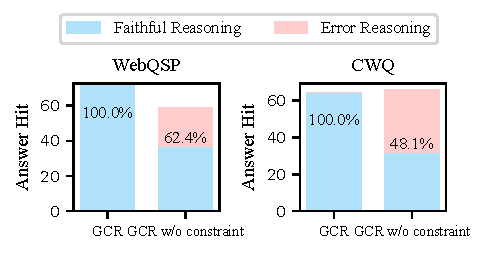
\includegraphics[width=.85\columnwidth]{images/exp_hallu_ratio.pdf}
      \end{center}
      \vspace{-14pt}
      \caption{Analysis of performance and reasoning errors in \ourmethod.}
      \vspace{-14pt}
    \label{fig:exp_hallucination_ratio}
\end{figure}
% \end{wrapfigure}
In this section, we investigate the effectiveness of KG constraints in eliminating hallucinations and ensuring faithful reasoning. We first compare the difference of answer accuracy (Hit) and \emph{faithful reasoning ratio} by removing KG constraints in graph-constrained decoding. The faithful reasoning ratio is calculated as the percentage of faithful reasoning in \emph{correctly predicted answers}. We define a reasoning as faithful where the generated reasoning path can be found in KGs, and vice versa. 

From the \Cref{fig:exp_hallucination_ratio}, we can observe that \ourmethod achieves the 100\% faithful reasoning ratio on both datasets, which indicates that \ourmethod can eliminate hallucinations and ensure faithful reasoning during reasoning on KGs. In contrast, when removing KG constraints, both the answer accuracy and faithful reasoning decrease significantly on WebQSP. This shows that KG constraints not only improve reasoning by reducing the searching space, but also play a crucial role in preventing hallucinations for accurate reasoning. While the answer hit rate on CWQ remains almost unchanged, the ratio of faithful reasoning still decreases to 48.1\%. This implies that even if LLMs can produce correct answers, the reasoning process is still prone to hallucinations and cannot be trusted, which is aligned with the findings in previous studies \citep{nguyen-etal-2024-direct}.

\begin{table*}[]
    \centering
    \caption{Examples of the faithful reasoning conducted by \ourmethod. \textcolor{red}{Red} denotes the incorrect reasoning paths and answers, while \textbf{bold} denotes the correct paths and answers.}
    % \vspace{-0.3cm}
    \label{tab:cases}
    \resizebox{.82\textwidth}{!}{%
    \begin{tabular}{@{}c|p{5in}@{}}
        \toprule
        \multicolumn{2}{l}{\textbf{Case 1}: Incorrect answers and hallucinated reasoning paths without constraints.}\\
        \midrule
        Question             & Who is niall ferguson 's wife?                                                                                                                                                                                                                                                                                             \\ \midrule
        Answer               & Ayaan Hirsi Ali                                                                                                                                                                                                                                                                                                                                \\ \midrule
        \ourmethod   $w/o$ constraint        & \begin{tabular}[c]{@{}p{5in}@{}}\# Reasoning Path: \textcolor{red}{Niall Ferguson $\to$ people.person.children $\to$ Mabel Rose Ferguson $\to$ people.person.parents $\to$ Alyssa Mastromonaco} \\ \#Answer: \textcolor{red}{Alyssa Mastromonaco}\end{tabular} \\\midrule
        \ourmethod                                   & \begin{tabular}[c]{@{}p{5in}@{}}\# Reasoning Path: Niall Ferguson $\to$ people.person.children $\to$ Thomas Ferguson $\to$ people.person.parents $\to$ \textbf{Ayaan Hirsi Ali} \\ \#Answer: \textbf{Ayaan Hirsi Ali} \end{tabular} \\ \midrule\midrule
        \multicolumn{2}{l}{\textbf{Case 2}: Correct answers but hallucinated reasoning paths without constraints.}\\\midrule
        Question             & Where is jamarcus russell from?                                                                                                                                                                                                                                                                                 \\ \midrule
        Answer               & Mobile                                                                                                                                                                                                                                                                                                                                                \\ \midrule
        \ourmethod   $w/o$ constraint        & \begin{tabular}[c]{@{}p{5in}@{}}\# Reasoning Path: \textcolor{red}{JaMarcus Russell $\to$ people.person.place\_of\_birth $\to$ Tampa} \\ \#Answer: \textbf{Mobile, Alabama} \end{tabular} \\\midrule
        \ourmethod                                   & \begin{tabular}[c]{@{}p{5in}@{}}\# Reasoning Path: JaMarcus Russell $\to$ people.person.place\_of\_birth $\to$ \textbf{Mobile} \\ \#Answer: \textbf{Mobile} \end{tabular} \\ 
        \bottomrule
    \end{tabular}}
    % \vspace{-0.5cm}
\end{table*}




\noindent\textbf{Case Study.} We further provide a case study to illustrate the effectiveness of \ourmethod in eliminating hallucinations and ensuring faithful reasoning. As shown in \Cref{tab:cases}, the first case demonstrates that, without constraints, the model generates an incorrect reasoning path leading to an incorrect answer by hallucinating facts such as ``Mabel Rose Ferguson is the child of Naill Ferguson and her parent is Alyssa Mastromonaco''. In contrast, \ourmethod generates a faithful reasoning path grounded in KGs that ``Naill Ferguson has a child named Thomas Ferguson who has a parent named Ayaan Hirsi Ali''. Based on the paths we can reason the correct answer to the question is ``Ayaan Hirsi Ali''. In the second case, although the LLM answers the question correctly, the generated reasoning path is still hallucinated with incorrect facts. Conversely, \ourmethod conducts faithful reasoning with both correct answer and reasoning path. These results demonstrate that \ourmethod can effectively eliminate hallucinations and ensure faithful reasoning by leveraging KG constraints in graph-constrained decoding.

\subsection{RQ3: Zero-shot Generalizability to Unseen KGs}\label{sec:transferability}
In \ourmethod, the knowledge graph is converted into a constraint which is plugged into the decoding process of LLMs. This allows \ourmethod to generalize to unseen KGs without further training. To evaluate the generalizability of \ourmethod, we conduct zero-shot transfer experiments on \RE{three} unseen KGQA datasets: \RE{FreebaseQA \citep{jiang2019freebaseqa}}, CSQA \citep{talmor2019commonsenseqa} and MedQA \citep{jin2021disease}. Specifically, we use the same KG-specialized LLM (Llama-3.1-8B) trained on Freebase as well as two general LLMs (ChatGP, GPT-4o-mini). During reasoning, we directly plug the KG-Trie constructed from \RE{Freebase}, ConceptNet and medical KGs into the \ourmethod to conduct graph-constrained decoding without additional fine-tuning. The results are shown in \Cref{tab:transferability}. 
%\reza{Reza: what if we use an 'untrained' model together with the constrained decoding for path generation in Table 6 (ie GCR without training the specialized model)? (probably it's much lower, and then it highlights the importance of transfer learning)}

% Please add the following required packages to your document preamble:
% \usepackage{booktabs}
% \usepackage{graphicx}\

% \begin{wraptable}{r}{0.6\columnwidth}
\begin{table}
    \centering
    \vspace{-0.4cm}
    \caption{Zero-shot transferability to other KGQA datasets.}
    \label{tab:transferability}
    % \vspace{-0.3cm}
    \resizebox{0.8\columnwidth}{!}{%
    \begin{tabular}{@{}cccc@{}}
    \toprule
    Model       & \RE{FreebaseQA} & CSQA & MedQA \\ \midrule
    ChatGPT     & \RE{85} & 79   & 64    \\
    \ourmethod (ChatGPT) & \RE{\textbf{92}} & \textbf{85}   & \textbf{66}    \\ \midrule
    GPT-4o-mini     & \RE{89} & 91   & 75    \\
    \ourmethod (GPT-4o-mini) & \RE{\textbf{94}} & \textbf{94}   & \textbf{79}    \\ \bottomrule
    \end{tabular}%
    }
    \vspace{-0.3cm}
% \end{wraptable}
\end{table}
From the results, it is evident that \ourmethod outperforms ChatGPT and GPT-4o-mini in zero-shot performance on both datasets. \RE{Specifically, \ourmethod shows 8.2\% and 7.6\% increase in accuracy on FreebaseQA and CSQA, respectively.} This highlights the strong zero-shot generalizability of its graph reasoning capabilities to unseen datasets and KGs without additional training. However, the improvement on MedQA is not as significant as that on CSQA. We hypothesize this difference may be due to LLMs having more common sense knowledge, which aids in reasoning on common sense knowledge graphs effectively. On the other hand, medical KGs are more specialized and require domain-specific knowledge for reasoning, potentially limiting the generalizability of our method.
